\documentclass[11pt,a4paper]{article}

\usepackage[utf8]{inputenc}
\usepackage[T1]{fontenc}
\usepackage{babel}
\babelprovide[main,import]{spanish}
\usepackage{lmodern}
\usepackage[a4paper,margin=2.35cm]{geometry}
\usepackage{amsmath,amssymb}
\usepackage{booktabs}
\usepackage{caption}
\usepackage{enumitem}
\usepackage{float}
\usepackage{graphicx}
\usepackage{xcolor}
\usepackage{listings}
\usepackage{microtype}
\usepackage{hyperref}

\graphicspath{{figures/shap/}{figures/inputs/}}
\hypersetup{
  colorlinks=true,
  linkcolor=blue!55!black,
  citecolor=blue!55!black,
  urlcolor=blue!65!black,
  pdftitle={Qué mira una CNN de vehículos: explicación local con SHAP},
  pdfauthor={REI-Tarea-AsistDev}
}

\emergencystretch=2em

\definecolor{codegray}{RGB}{245,245,245}
\lstset{
  language=Python,
  basicstyle=\ttfamily\footnotesize,
  backgroundcolor=\color{codegray},
  frame=single,
  rulecolor=\color{black!20},
  breaklines=true,
  keepspaces=true,
  columns=fullflexible,
  showstringspaces=false
}

\title{\textbf{¿Qué mira una CNN de vehículos?\\ explicación local y reproducible con SHAP}}
\author{REI\_Tarea\_AsistDev}
\date{4 de septiembre de 2026}

\begin{document}

\maketitle

\begin{abstract}
Este trabajo aplica SHAP (\emph{SHapley Additive exPlanations}) a una red
neuronal convolucional que clasifica imágenes de vehículos en siete clases.
El objetivo no es solamente mostrar la clase predicha, sino localizar qué
regiones aumentan o disminuyen la probabilidad de esa salida. Se usa un
\emph{Partition explainer} con un enmascarador de imagen por desenfoque y se
verifica la propiedad aditiva de las atribuciones. En una muestra de tres
imágenes, la bicicleta correcta recibe apoyo principalmente en regiones que
contienen cuadro y rueda; en los dos errores, las atribuciones muestran que el
contexto y las texturas de la escena también pueden mover la predicción. Estos
resultados son locales: no deben confundirse con una importancia global del
modelo ni con porcentajes semánticos de “ruedas” o “casco”. Todo el código,
modelo, figuras y este documento están disponibles en el repositorio
\href{https://github.com/nel-eleven11/REI_Tarea_AsistDev}{GitHub del proyecto}.
\end{abstract}

\section{Motivación y pregunta}

Una probabilidad de salida responde \emph{qué} decidió el modelo, pero no
explica \emph{por qué}. En clasificación visual, la pregunta natural es:

\begin{quote}
\textbf{¿Qué regiones de cada imagen favorecen o contradicen la clase
predicha, y el clasificador parece usar el vehículo o el contexto de la
escena?}
\end{quote}

SHAP emplea valores de Shapley para repartir la diferencia entre una predicción
y una referencia entre las características. En este caso una característica
no es una palabra o una columna tabular: es una región espacial de la imagen
que el enmascarador puede ocultar. Por tanto, una atribución roja significa que
la región empuja la probabilidad de la clase explicada hacia arriba; una azul,
que la empuja hacia abajo. El objetivo es diagnosticar el comportamiento del
modelo, no demostrar causalidad sobre el objeto real.

\section{Materiales y configuración reproducible}

\subsection{Modelo y datos}

El punto de partida es el notebook
\texttt{vehicle-image-classification-using-cnn.ipynb}. El dataset local
\texttt{Vehicles/} contiene siete directorios: \textit{Auto Rickshaws},
\textit{Bikes}, \textit{Cars}, \textit{Motorcycles}, \textit{Planes},
\textit{Ships} y \textit{Trains}. Con semilla 42, se separan los ejemplos por
clase en 80\% para entrenamiento y 20\% para validación. El notebook informa
4\,454 imágenes de entrenamiento, 1\,114 de validación y 22 archivos
incompatibles excluidos por firma binaria. Las imágenes se redimensionan a
128$\times$128 píxeles RGB.

La CNN tiene tres capas convolucionales de 32, 64 y 128 filtros, cada una
seguida por max-pooling, global average pooling, una capa densa de 128
unidades y una salida softmax de siete clases. Durante entrenamiento se usan
volteo horizontal, rotación y zoom como aumento de datos, además de
\texttt{Rescaling(1/255)}. Se entrenó por tres épocas con Adam y
\texttt{categorical\_crossentropy}; la evaluación conservada en el notebook
reporta pérdida de validación 1.4443 y exactitud 43.00\%.

\subsection{Muestras de explicación}

Se conservan tres entradas exportadas del panel de validación del notebook:
un tren etiquetado como \textit{Trains} pero predicho como \textit{Cars}, un
barco etiquetado como \textit{Ships} pero predicho como \textit{Planes}, y una
bicicleta etiquetada y predicha como \textit{Bikes}. Esto permite contrastar
dos errores con un acierto sin ocultar que son solamente tres casos.

\subsection{Configuración de SHAP}

Se ejecuta SHAP 0.46.0 con TensorFlow CPU 2.18.1. El enmascarador de imágenes
de SHAP reemplaza particiones por una versión desenfocada con bloques de
32$\times$32 píxeles (la clase usada es \texttt{Image}). El explainer particiona la imagen y estima
las atribuciones con 300 evaluaciones por muestra; se fija la semilla en 42.
La selección \texttt{shap.Explanation.argsort.flip[:1]} explica la salida más
alta de cada imagen, es decir, la clase que el propio modelo predijo. La
elección de un enmascarador de imagen y la visualización de salidas para
clasificación siguen los ejemplos de la documentación oficial de SHAP
\cite{shap_image_docs}; la definición de SHAP se basa en Lundberg y Lee
\cite{lundberg2017unified}. La preparación de un clasificador de imágenes
convolucional sigue el flujo habitual de TensorFlow para este tipo de tarea
\cite{tensorflow_image_classification}.

Para una entrada $x$, la comprobación numérica usada es
\begin{equation}
  f_k(x) = b_k(x) + \sum_{i=1}^{m}\phi_{i,k}(x),
  \label{eq:additivity}
\end{equation}
donde $f_k(x)$ es la probabilidad de la clase $k$, $b_k(x)$ es la salida con
la referencia enmascarada y $\phi_{i,k}$ es la contribución de la partición
$i$. En imágenes RGB se guardan las atribuciones por canal; para resumir una
región espacial se suman sus tres canales. La figura de color se normaliza por
muestra solamente para hacer visibles las diferencias locales.

\section{Resultados}

\subsection{Predicción y regiones dominantes}

La Tabla~\ref{tab:predictions} resume la salida que se obtuvo al volver a
ejecutar el análisis sobre el modelo versionado. ``Base'' es $b_k(x)$ y no es
la confianza de la imagen original. ``Top $|\text{SHAP}|$'' es la región 4$\times$4
con mayor suma de atribuciones absolutas; su porcentaje se calcula dentro de
esa imagen y sirve para ordenar regiones, no para declarar que una parte
semántica del vehículo explica exactamente ese porcentaje.

\begin{table}[H]
\centering
\caption{Predicciones y concentración espacial de la atribución.}
\label{tab:predictions}
\small
\begin{tabular}{@{}llllrr@{}}
\toprule
Muestra & Real & Predicción & $p_k$ & Base & Top $|\text{SHAP}|$ \\
\midrule
Tren & Trains & Cars & 0.223 & 0.167 & inferior-centro-izquierda (38.7\%) \\
Barco & Ships & Planes & 0.522 & 0.562 & inferior-izquierda (39.6\%) \\
Bicicleta & Bikes & Bikes & 0.643 & 0.235 & medio-inferior-centro-derecha (16.0\%) \\
\bottomrule
\end{tabular}
\end{table}

En el tren, la atribución positiva se concentra en la parte baja izquierda,
que incluye el frente del tren y texturas de vía/plataforma en la imagen
redimensionada. Esa evidencia local empuja Cars desde una base de 0.167 hasta
0.223; no basta para afirmar que el modelo haya aprendido “ruedas de auto”.
En el barco, la salida Planes parte de una base alta de 0.562 y las
atribuciones negativas totalizan aproximadamente $-0.0406$; el casco, la
vegetación y la zona inferior contradicen parcialmente esa salida, pero no lo
suficiente para cambiar la clase. En la bicicleta, las atribuciones positivas
se distribuyen sobre el cuadro, las ruedas y el manubrio; la clase pasa de
0.235 a 0.643.

\begin{figure}[H]
\centering
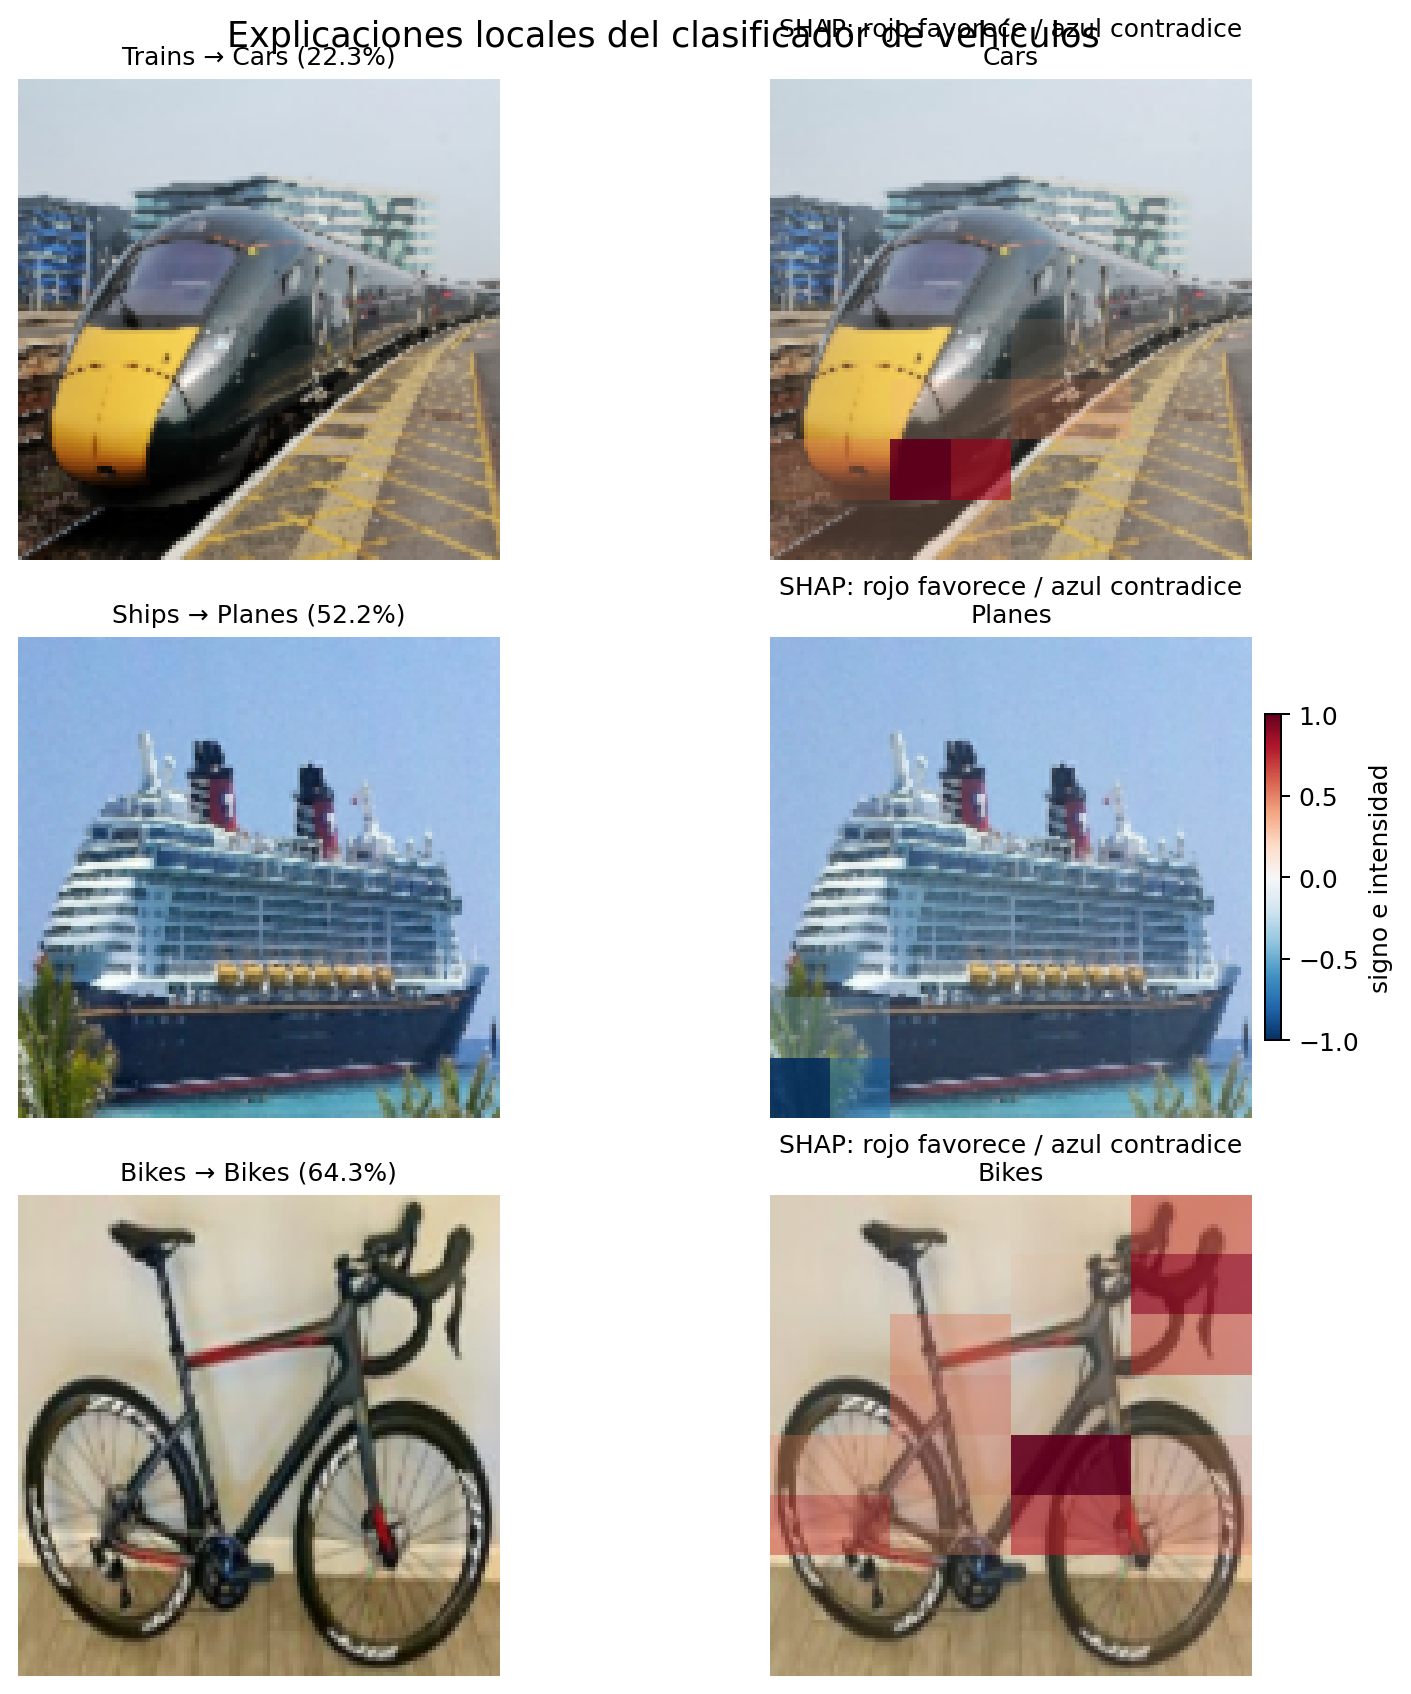
\includegraphics[width=0.92\linewidth]{shap_overview.png}
\caption{Entrada y mapa SHAP para la clase predicha. Rojo favorece la clase
explicada; azul la contradice. La intensidad está normalizada dentro de cada
muestra para mejorar la lectura visual.}
\label{fig:overview}
\end{figure}

\subsection{Evidencia local de los tres casos}

Las figuras individuales muestran la entrada, el mapa de atribución sobre la
imagen y la suma de $|\text{SHAP}|$ en una cuadrícula 4$\times$4. La cuadrícula
es una agregación espacial reproducible, no una segmentación de “vehículo” y
“fondo”.

\begin{figure}[H]
\centering
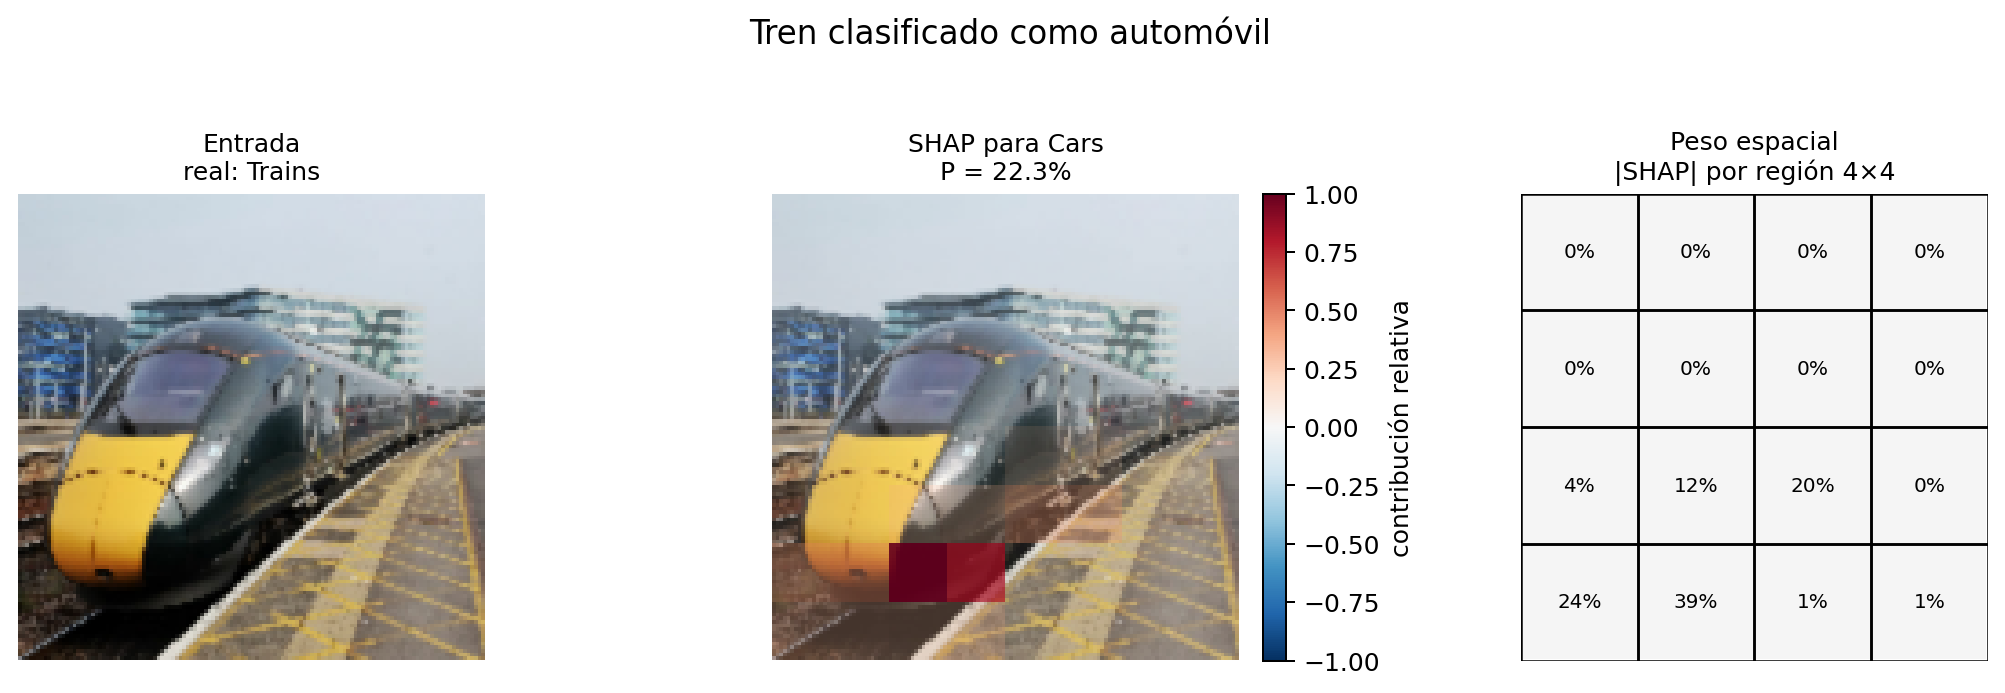
\includegraphics[width=0.98\linewidth]{train_misclassified_shap.png}
\caption{Tren real, predicho como Cars. La evidencia positiva se concentra en
la zona inferior izquierda/central de esta entrada.}
\label{fig:train}
\end{figure}

\begin{figure}[H]
\centering
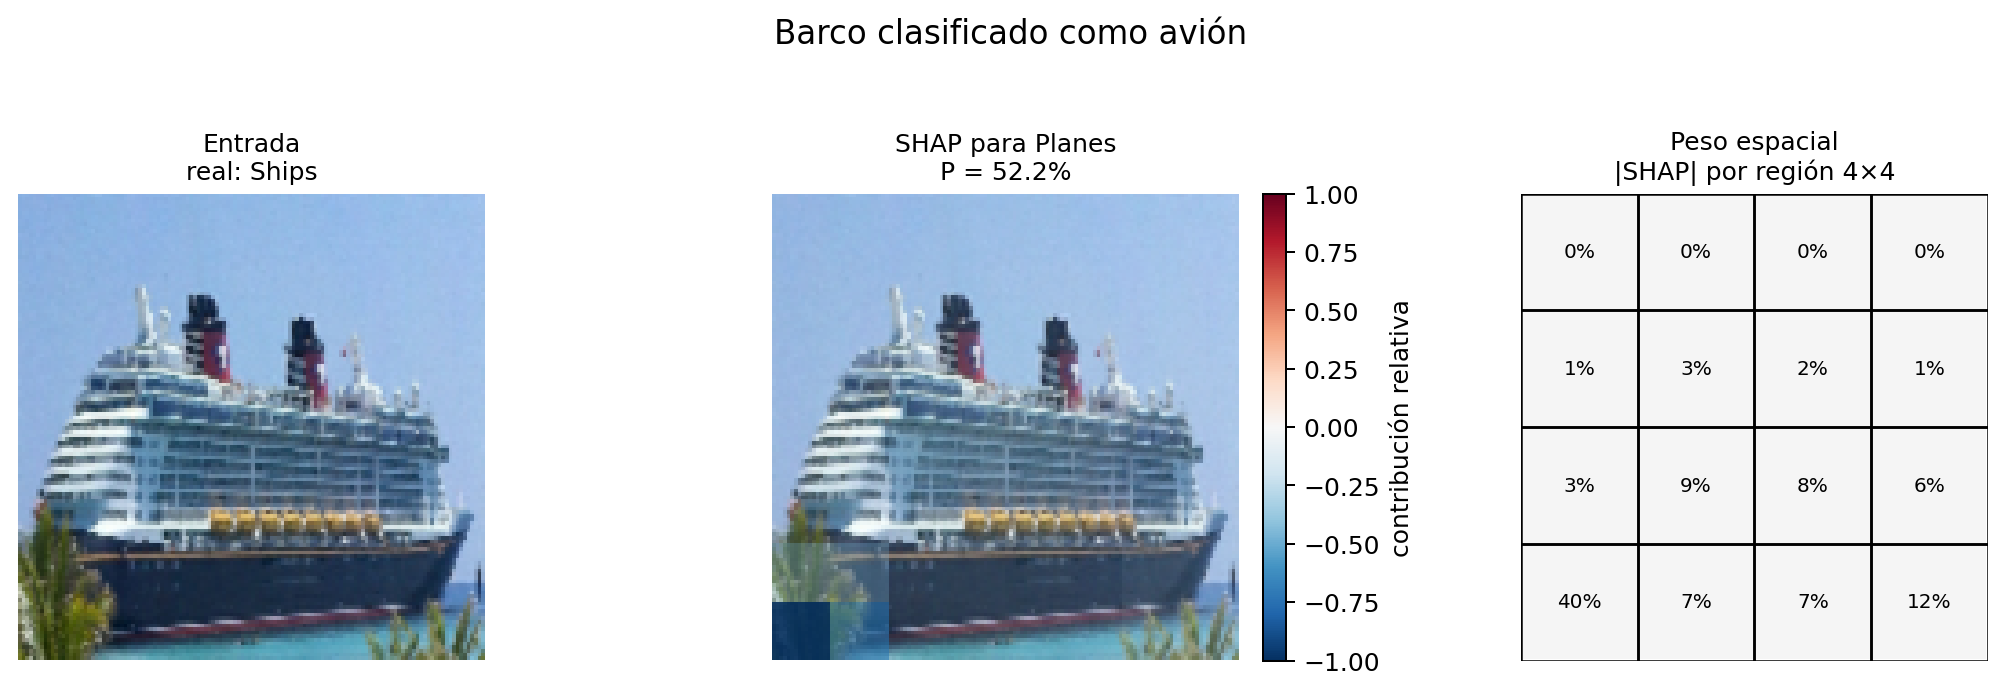
\includegraphics[width=0.98\linewidth]{ship_misclassified_shap.png}
\caption{Barco real, predicho como Planes. La masa negativa domina; el mapa
identifica regiones que reducen la probabilidad de Planes sin que la clase
correcta llegue a ser la máxima.}
\label{fig:ship}
\end{figure}

\begin{figure}[H]
\centering
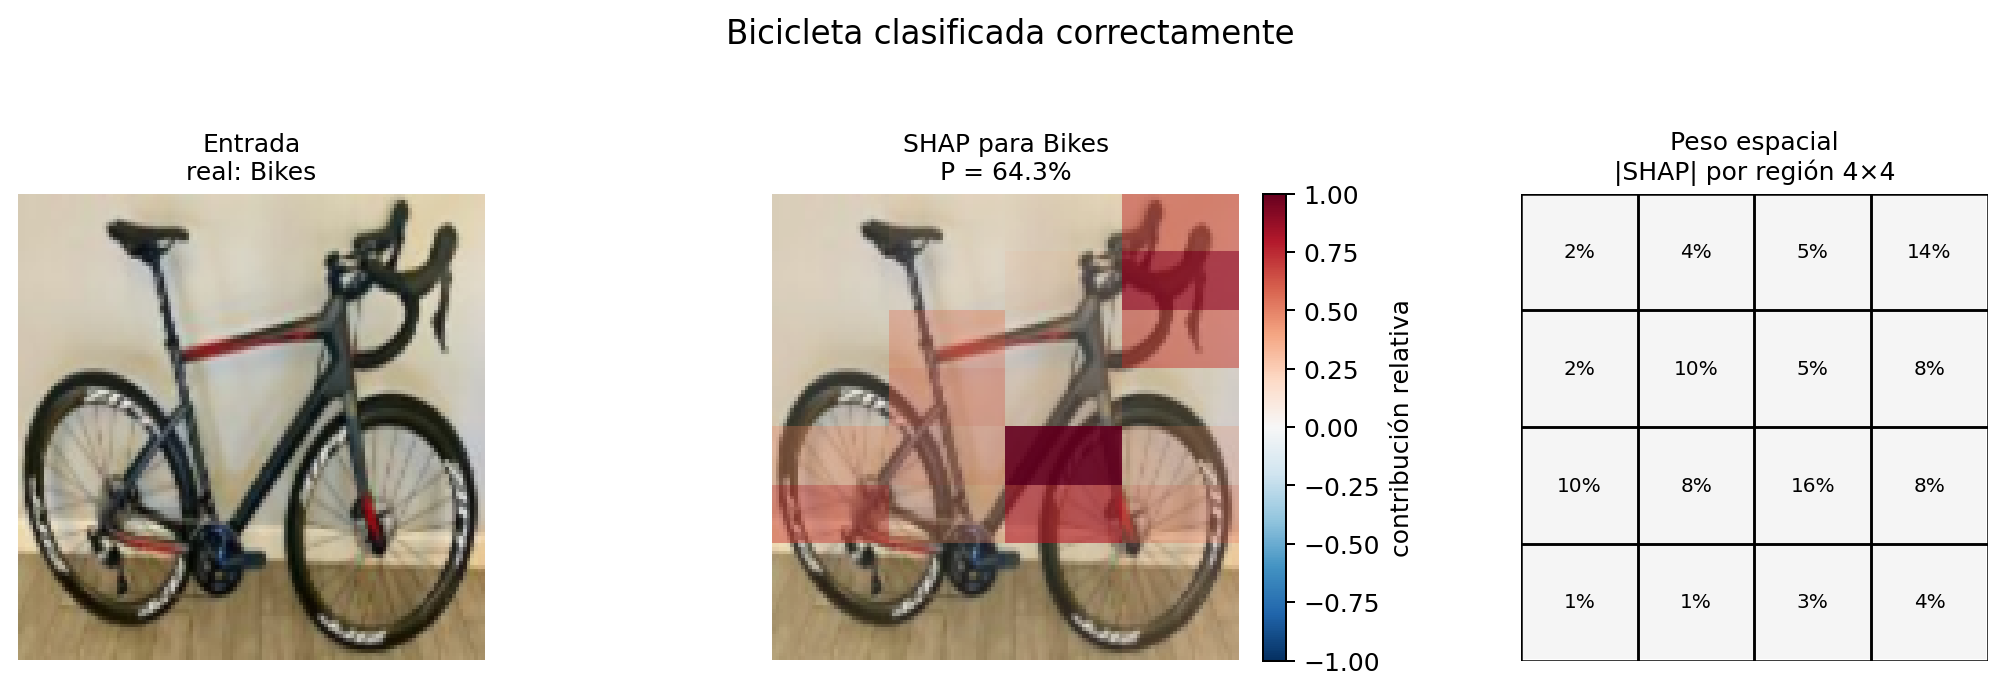
\includegraphics[width=0.98\linewidth]{bike_correct_shap.png}
\caption{Bicicleta clasificada correctamente como Bikes. El cuadro, las ruedas
y el manubrio aparecen entre las zonas con mayor atribución local.}
\label{fig:bike}
\end{figure}

\subsection{Resumen agregado de la muestra}

La Figura~\ref{fig:global} suma la magnitud absoluta de las atribuciones de
las tres imágenes. El resultado sugiere que las zonas medio-inferior y
superior-derecha aparecen con frecuencia en esta pequeña selección, pero no
es una medida global de todo el dataset: cambiar las tres imágenes puede
cambiar el ranking. Para una conclusión global se necesitaría explicar una
muestra grande y resumir por clase, con intervalos de variabilidad.

\begin{figure}[H]
\centering
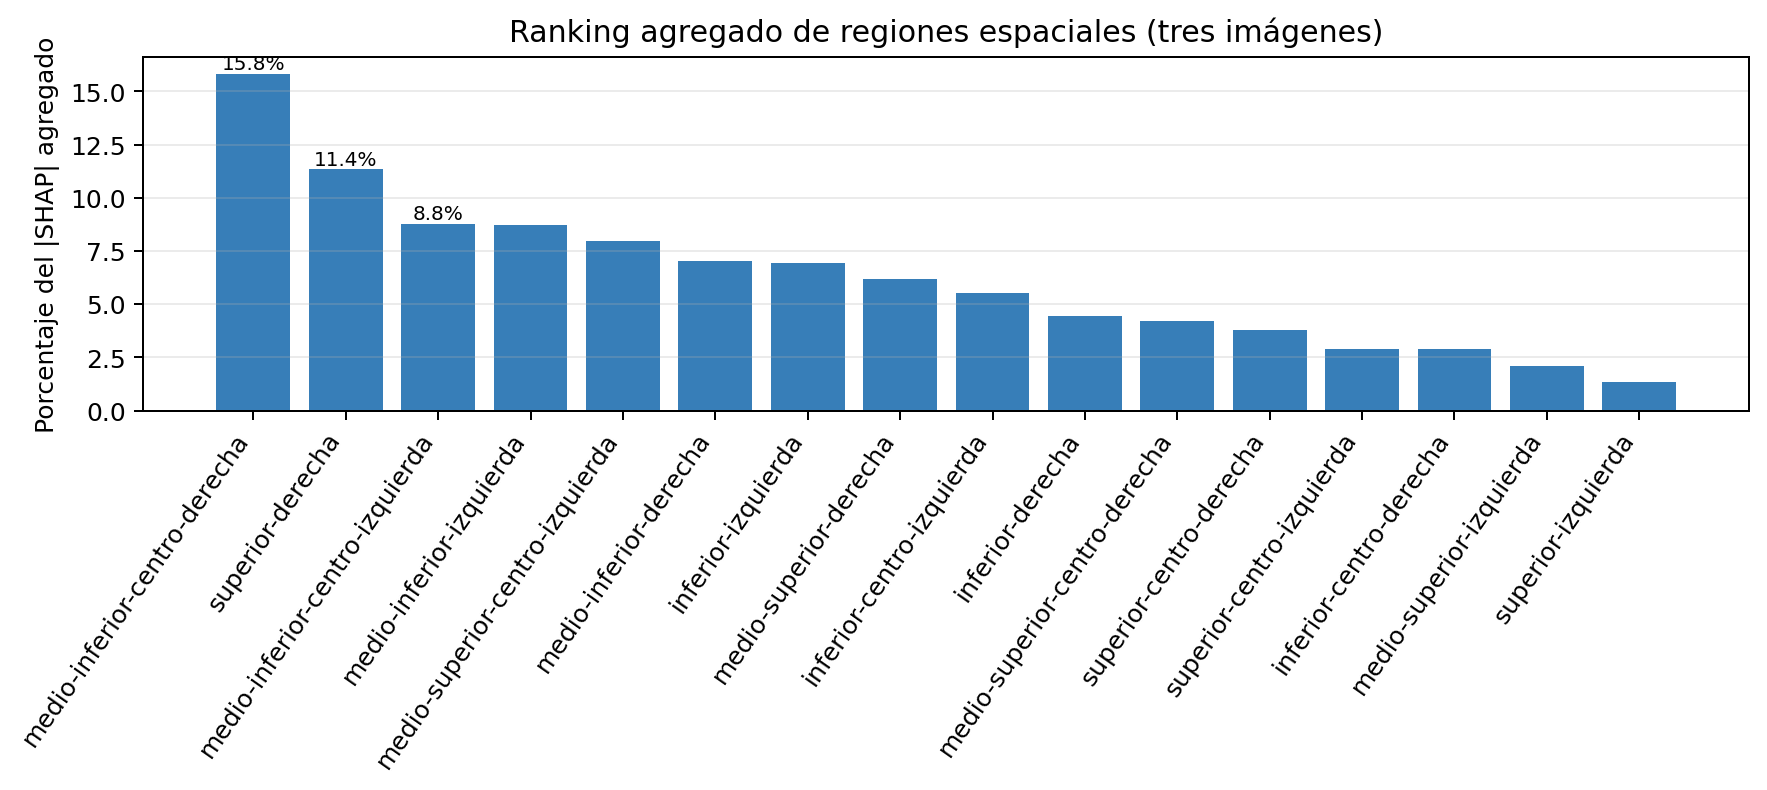
\includegraphics[width=0.97\linewidth]{global_region_importance.png}
\caption{Ranking agregado de regiones 4$\times$4 en las tres imágenes. Cada
barra es porcentaje de $|\text{SHAP}|$ agregado, no probabilidad.}
\label{fig:global}
\end{figure}

\subsection{Comprobación de aditividad}

En las tres muestras la suma de la base y las atribuciones coincide con la
probabilidad de la salida explicada al nivel mostrado por la ejecución:
el error fue $0.00\times10^{0}$ en el CSV generado. Esto confirma que el mapa
describe la salida seleccionada por el explainer; no confirma que la
explicación sea causal ni que el modelo sea correcto.

\section{Reproducibilidad y paquete entregable}

El URL canónico del proyecto, incluido también en el resumen, es:
\begin{center}
\url{https://github.com/nel-eleven11/REI_Tarea_AsistDev}
\end{center}

Desde la raíz del repositorio, el flujo completo es:

\begin{lstlisting}
uv venv --python 3.10 .venv
uv pip install --python .venv/bin/python -r requirements-shap.txt
.venv/bin/python shap_analysis.py
pdflatex paper.tex
bibtex paper
pdflatex paper.tex
pdflatex paper.tex
\end{lstlisting}

El script escribe resultados JSON, CSV y NPZ dentro de
\texttt{figures/shap/}, además del resumen visual y una figura por caso. El
dataset completo no se versiona por tamaño; el
notebook conserva el procedimiento para reentrenar si se dispone de
\texttt{Vehicles/}. Las tres imágenes usadas en este paper sí están
versionadas, por lo que el resultado SHAP no depende de descargar datos
externos.

Existe una consideración de portabilidad: el archivo \texttt{.keras} registra una
versión de Keras más nueva que la del entorno CPU usado para ejecutar esta
entrega. \texttt{shap\_analysis.py} intenta la carga normal y tiene un fallback que
reconstruye la arquitectura conocida y carga únicamente los pesos internos;
el resultado de predicción se verifica antes de explicar.

\section{Limitaciones y trabajo futuro}

\begin{enumerate}[leftmargin=*]
  \item \textbf{Muestra pequeña.} Tres imágenes no permiten afirmar una
  regla universal del clasificador. El ranking agregado solamente describe
  este caso de estudio.
  \item \textbf{Regiones, no conceptos.} Una celda 4$\times$4 mezcla partes
  del vehículo y el fondo. Para responder literalmente cuánto pesan ruedas,
  ventanas u orejas se necesita una segmentación o anotaciones semánticas y
  una definición de agregación antes de calcular SHAP.
  \item \textbf{Dependencia del enmascarador.} Cambiar de desenfoque a
  inpainting, el tamaño de partición o el número de evaluaciones puede cambiar
  la distribución espacial. El mapa es relativo a la referencia elegida.
  \item \textbf{Modelo modesto.} La exactitud de validación es 43.00\% y la
  muestra contiene dos errores. Las explicaciones ayudan a diagnosticar, pero
  no convierten al modelo en un sistema apto para decisiones críticas.
  \item \textbf{Confianza.} SHAP reparte cambios en la salida del modelo; una
  atribución de 0.04 no significa que la imagen tenga 4\% de probabilidad de
  contener una parte. Probabilidad, atribución y porcentaje de masa absoluta
  son cantidades distintas.
\end{enumerate}

\section{Conclusión}

La inspección SHAP responde la pregunta de manera más precisa que una lista
de confianzas: muestra qué zonas apoyan la clase predicha y cuáles la
contradicen. En el caso estudiado, la bicicleta correcta recibe evidencia
distribuida sobre su estructura, mientras que los errores de tren y barco
revelan que las texturas de la escena pueden contribuir a una clase incorrecta.
La conclusión responsable es local y diagnóstica: el modelo parece usar
patrones visuales concretos, pero estas tres imágenes no permiten traducirlos
automáticamente en una tabla semántica de “orejas 60\%” o “patas 30\%”.

\bibliographystyle{plain}
\bibliography{references}

\end{document}
